\documentclass[a4paper,10pt]{article}
\usepackage[dvips]{color,graphicx}
\usepackage[dvips, bookmarks, colorlinks=false]{hyperref}


%opening
\title{Math508 Homework 10}
\author{Yu Huang}

\begin{document}

\maketitle

\begin{abstract}
Simple Kalman Filter
\end{abstract}

\section{Problem 1}
$X_0, V_1, W_0$ distributed as $N(0,1)$.

\subsection{Part a}
$N=200, \alpha=0.9, \epsilon=0.3, \delta=1$, see Figure~\ref{f1} and Figure~\ref{f2}.

\begin{figure}
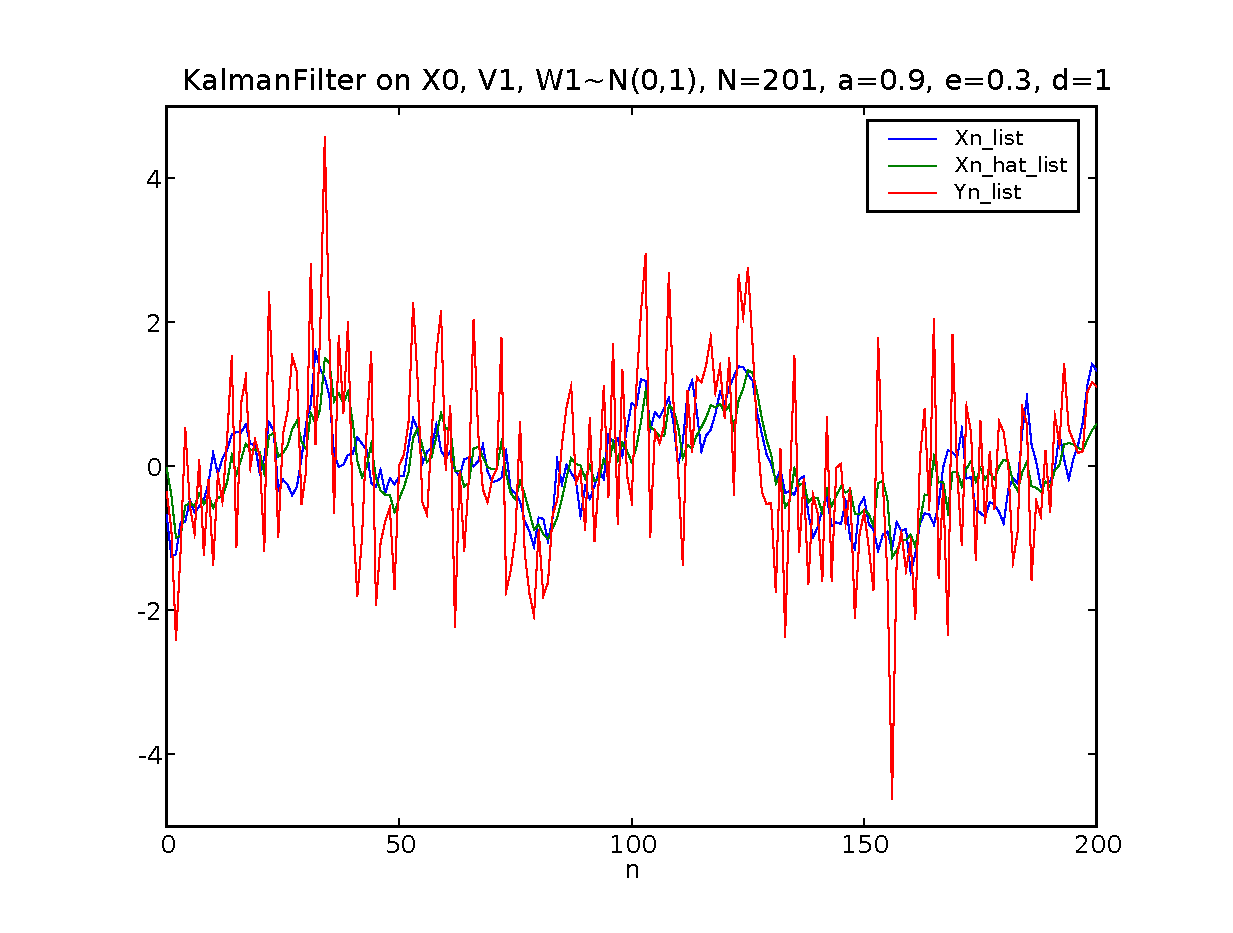
\includegraphics[width=1\textwidth]{hw10_1_N_201_a_0.9_e_0.3_d_1.eps}
\caption{}\label{f1}
\end{figure}

\begin{figure}
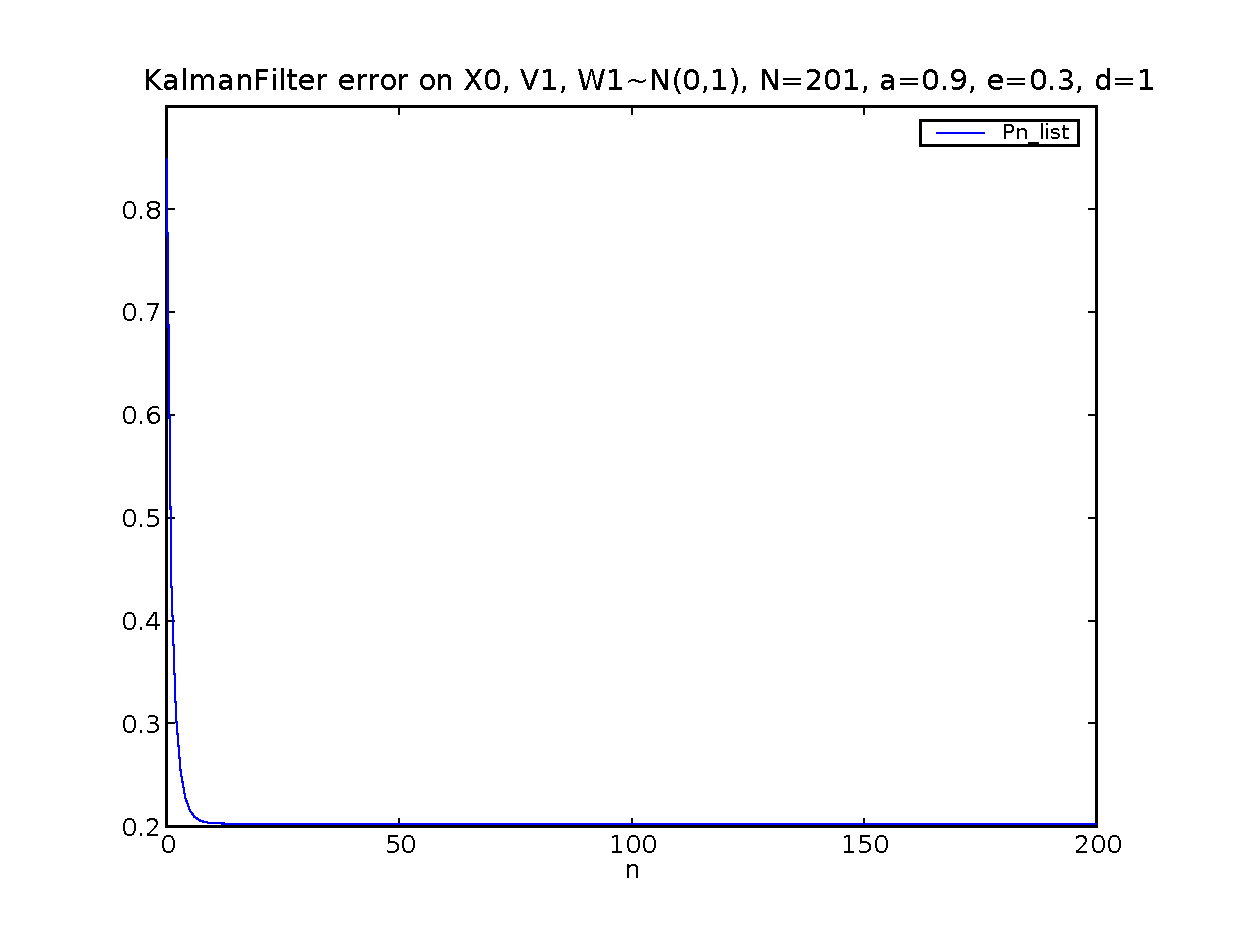
\includegraphics[width=1\textwidth]{hw10_1_error_N_201_a_0.9_e_0.3_d_1.eps}
\caption{}\label{f2}
\end{figure}


\subsection{Part b}
$N=200, \alpha=0.8, \epsilon=0.9, \delta=2$, see Figure~\ref{f3} and Figure~\ref{f4}.

\begin{figure}
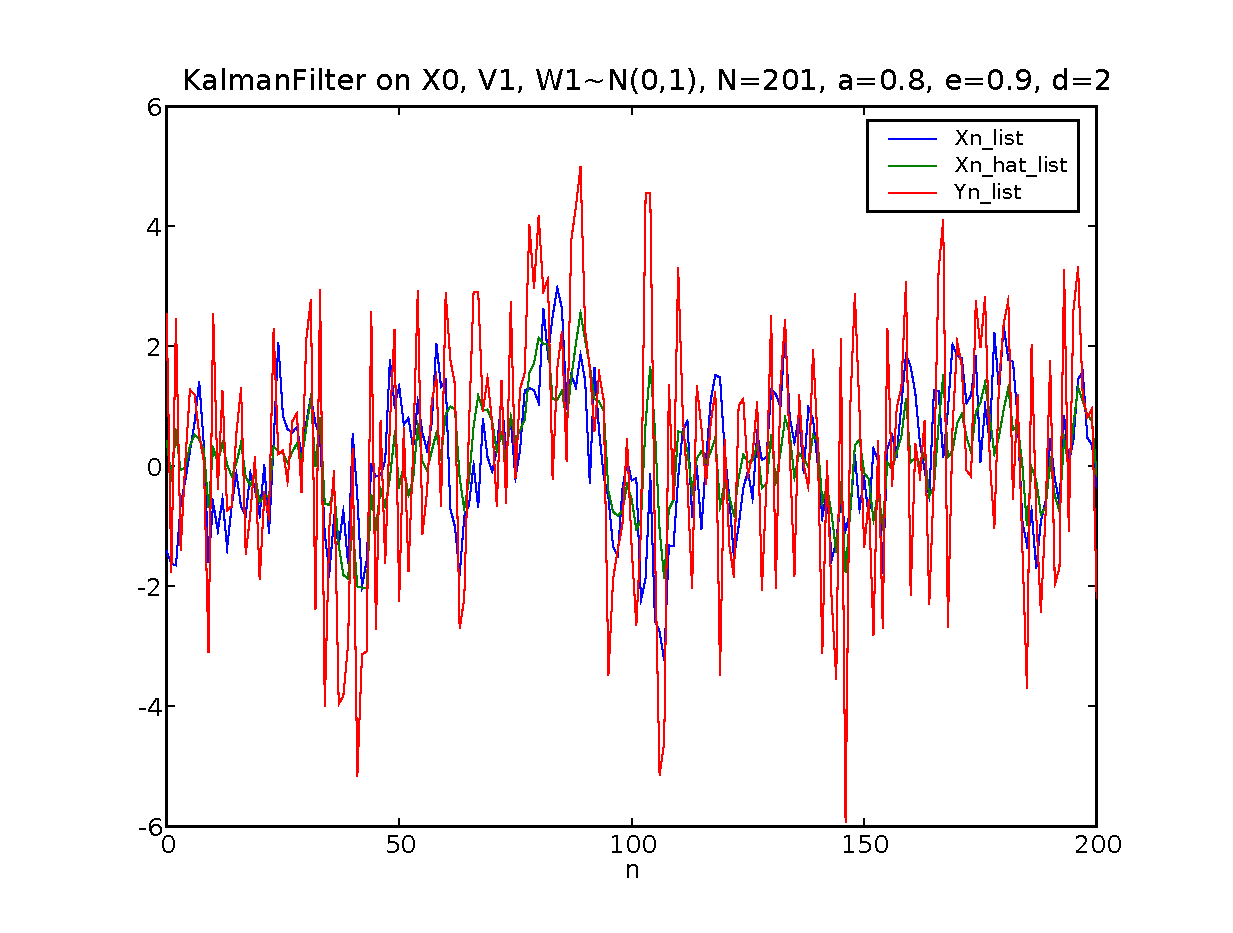
\includegraphics[width=1\textwidth]{hw10_1_N_201_a_0.8_e_0.9_d_2.eps}
\caption{}\label{f3}
\end{figure}

\begin{figure}
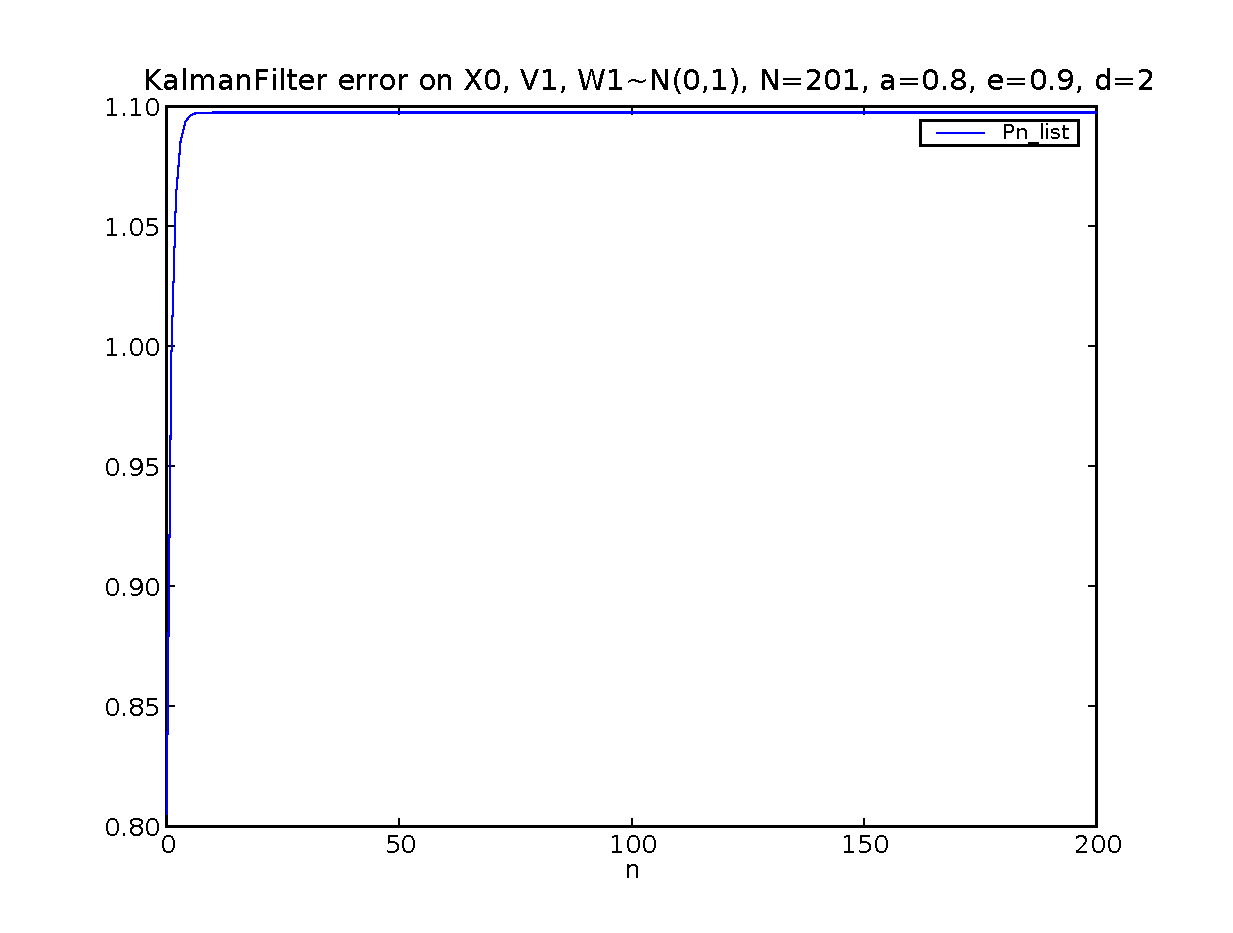
\includegraphics[width=1\textwidth]{hw10_1_error_N_201_a_0.8_e_0.9_d_2.eps}
\caption{}\label{f4}
\end{figure}

\section{Problem 2}
$X_0=1, P(V_1=\pm 1)=P(W_1=\pm 1)=\frac{1}{2}$.

$N=200, \alpha=0.9, \epsilon=0.3, \delta=1$, see Figure~\ref{f5} and Figure~\ref{f6}.

\begin{figure}
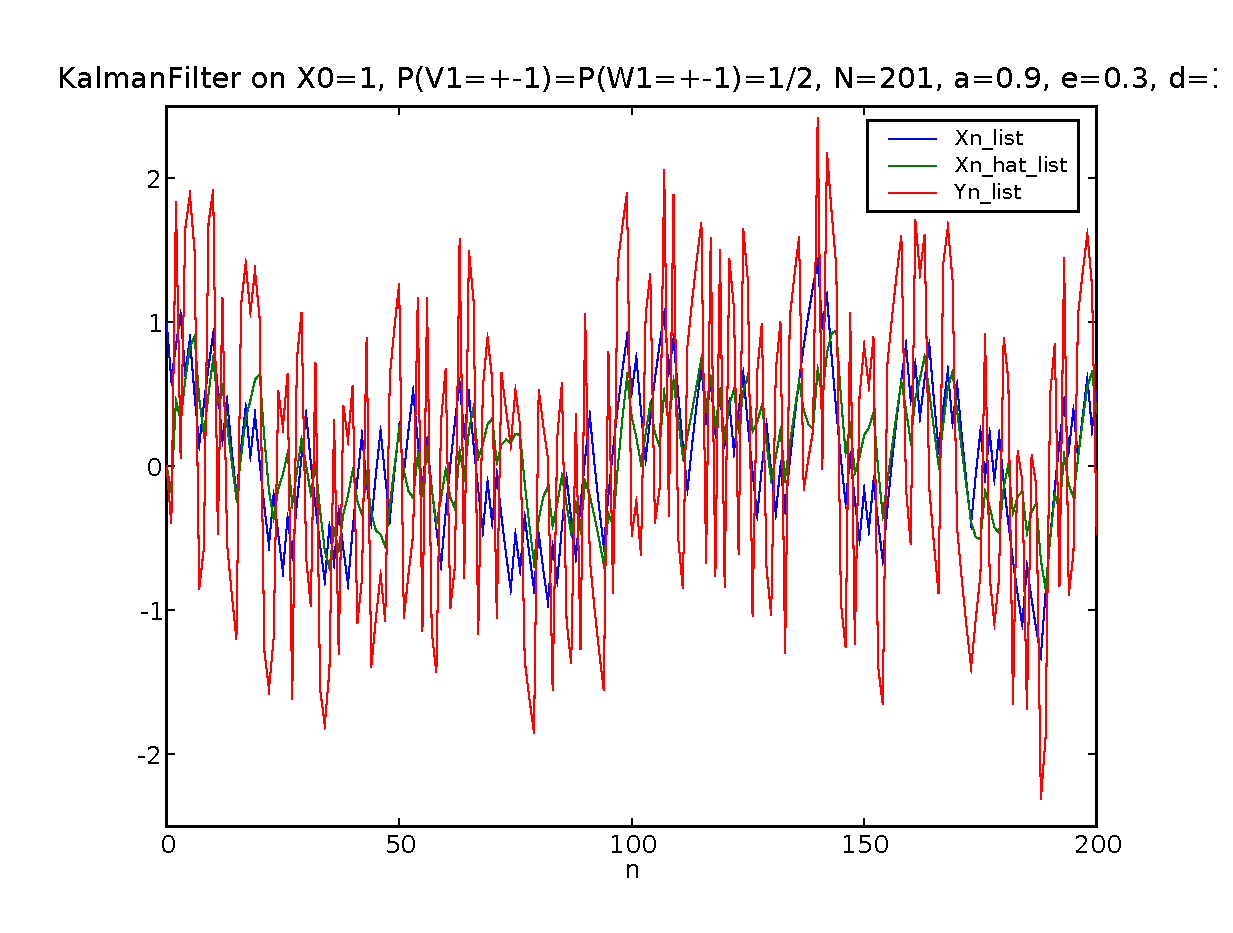
\includegraphics[width=1\textwidth]{hw10_2_N_201_a_0.9_e_0.3_d_1.eps}
\caption{}\label{f5}
\end{figure}

\begin{figure}
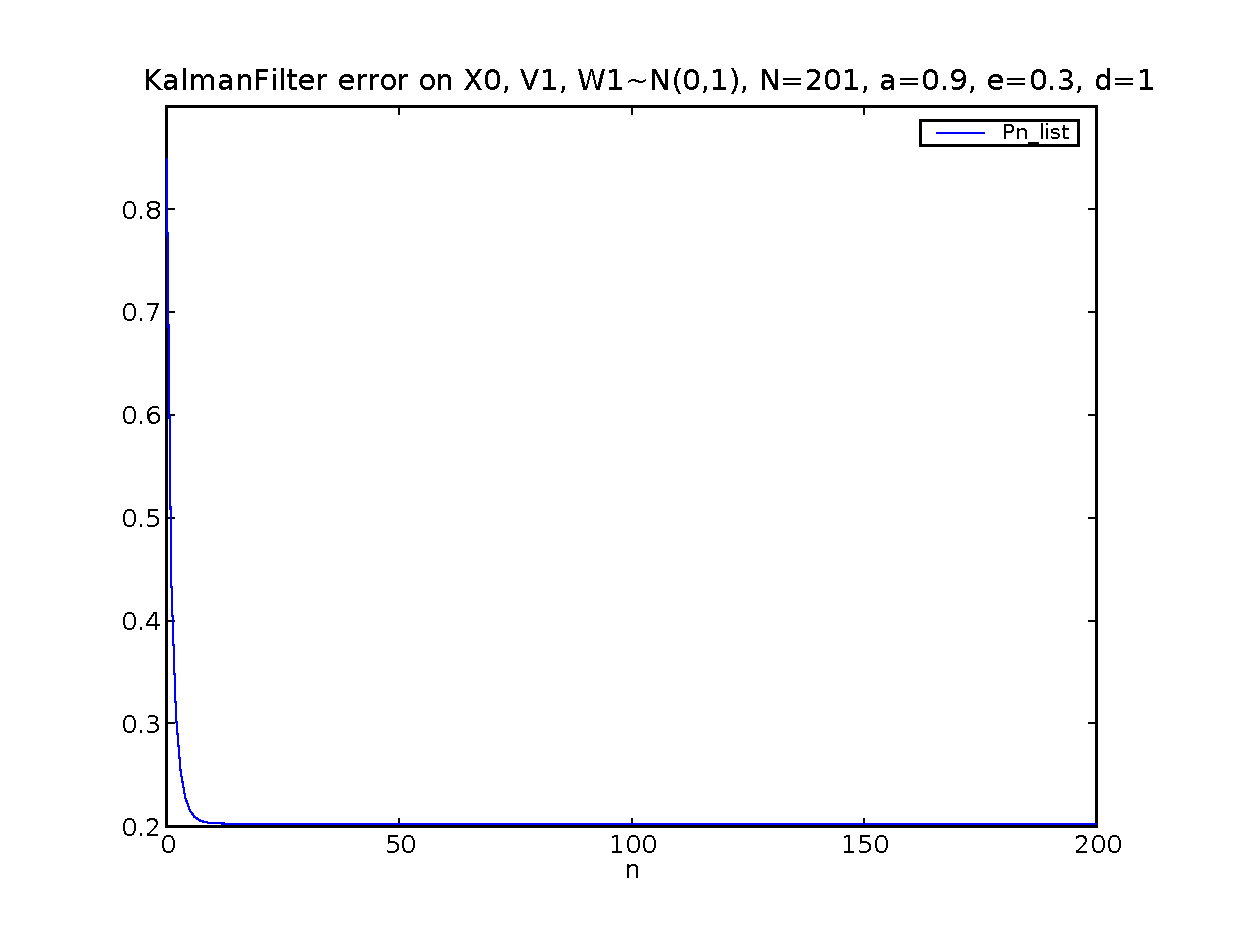
\includegraphics[width=1\textwidth]{hw10_2_error_N_201_a_0.9_e_0.3_d_1.eps}
\caption{}\label{f6}
\end{figure}

\end{document}
